%%%%%%%%%%%%%%%%%%%%%%%%%%%%%%%%%%%%%%%%%
% Programming/Coding Assignment
% LaTeX Template
%
% This template has been downloaded from:
% http://www.latextemplates.com
%
% Original author:
% Ted Pavlic (http://www.tedpavlic.com)
%
% Note:
% The \lipsum[#] commands throughout this template generate dummy text
% to fill the template out. These commands should all be removed when 
% writing assignment content.
%
% This template uses a Perl script as an example snippet of code,
% most other languages are also usable. Configure them in the
% "CODE INCLUSION CONFIGURATION" section.
%%%%%%%%%%%%%%%%%%%%%%%%%%%%%%%%%%%%%%%%%

%-------------------------------------------------------------------------
%	PACKAGES AND OTHER DOCUMENT CONFIGURATIONS
%-------------------------------------------------------------------------

\documentclass{article}

\usepackage{fancyhdr} % Required for custom headers
\usepackage{lastpage} % Required to determine the last page for the footer
\usepackage{extramarks} % Required for headers and footers
\usepackage[usenames,dvipsnames]{color} % Required for custom colors
\usepackage{graphicx} % Required to insert images
\usepackage{listings} % Required for insertion of code
\usepackage{courier} % Required for the courier font
\usepackage{hyperref}
\usepackage{amsmath}
\usepackage{bm}
\usepackage{mathrsfs}
\usepackage{float}
\usepackage{enumitem}
\usepackage[english]{babel}
\usepackage[utf8]{inputenc}
\usepackage{fontenc}
\usepackage{booktabs}
\usepackage{pdfpages}


% Margins
\topmargin=-0.45in
\evensidemargin=0in
\oddsidemargin=0in
\textwidth=6.5in
\textheight=9.0in
\headsep=0.25in

\linespread{1.1} % Line spacing

% Set up the header and footer
\pagestyle{fancy}
\lhead{\hmwkAuthorName} % Top left header
\chead{\hmwkClassShort\ (\hmwkClassInstructor)} % Top center head
%\rhead{\firstxmark} % Top right header
\rhead{\hmwkTitle}
\lfoot{\lastxmark} % Bottom left footer
\cfoot{} % Bottom center footer
% Bottom right footer
\rfoot{Page\ \thepage\ of\ \protect\pageref{LastPage}} 
\renewcommand\headrulewidth{0.4pt} % Size of the header rule
\renewcommand\footrulewidth{0.4pt} % Size of the footer rule

\setlength\parindent{0pt} % Removes all indentation from paragraphs

%--------------------------------------------------------------------------
%	CODE INCLUSION CONFIGURATION
%--------------------------------------------------------------------------
% This is the color used for comments
\definecolor{MyDarkGreen}{rgb}{0.0,0.4,0.0} 
\lstloadlanguages{Perl,Python} % Load Perl syntax for listings,
% for a list of other languages supported see:
%ftp://ftp.tex.ac.uk/tex-archive/macros/latex/contrib/listings/listings.pdf
\lstset{language=Perl, % Use Perl in this example
        frame=single, % Single frame around code
        basicstyle=\small\ttfamily, % Use small true type font
        keywordstyle=[1]\color{Blue}\bf, % Perl functions bold and blue
        keywordstyle=[2]\color{Purple}, % Perl function arguments purple
        % Custom functions underlined and blue
        keywordstyle=[3]\color{Blue}\underbar, 
        identifierstyle=, % Nothing special about identifiers
        % Comments small dark green courier font
        commentstyle=\usefont{T1}{pcr}{m}{sl}\color{MyDarkGreen}\small, 
        stringstyle=\color{Purple}, % Strings are purple
        showstringspaces=false, % Don't put marks in string spaces
        tabsize=5, % 5 spaces per tab
        %
        % Put standard Perl functions not included
        % in the default language here
        morekeywords={rand},
        %
        % Put Perl function parameters here
        morekeywords=[2]{on, off, interp},
        %
        % Put user defined functions here
        morekeywords=[3]{test},
       	%
        % Line continuation (...) like blue comment
        morecomment=[l][\color{Blue}]{...}, 
        numbers=left, % Line numbers on left
        firstnumber=1, % Line numbers start with line 1
        numberstyle=\tiny\color{Blue}, % Line numbers are blue and small
        stepnumber=5 % Line numbers go in steps of 5
}


\lstset{language=Python, % Use Python in this example
        frame=single, % Single frame around code
        basicstyle=\small\ttfamily, % Use small true type font
        keywordstyle=[1]\color{Blue}\bf, % Python functions bold and blue
        keywordstyle=[2]\color{Purple}, % Python function arguments purple
        % Custom functions underlined and blue
        keywordstyle=[3]\color{Blue}\underbar, 
        identifierstyle=, % Nothing special about identifiers
        % Comments small dark green courier font
        commentstyle=\usefont{T1}{pcr}{m}{sl}\color{MyDarkGreen}\small, 
        stringstyle=\color{Purple}, % Strings are purple
        showstringspaces=false, % Don't put marks in string spaces
        tabsize=3, % 5 spaces per tab
        %
        % Put standard Python functions not included in the
        % default language here
        morekeywords={rand},
        %
        % Put Python function parameters here
        morekeywords=[2]{on, off, interp},
        %
        % Put user defined functions here
        morekeywords=[3]{test},
       	%
        % Line continuation (...) like blue comment
        morecomment=[l][\color{Blue}]{...}, 
        numbers=left, % Line numbers on left
        firstnumber=1, % Line numbers start with line 1
        numberstyle=\tiny\color{Blue}, % Line numbers are blue and small
        stepnumber=5 % Line numbers go in steps of 5
}


% Creates a new command to include a perl script, the first
% parameter is the filename of the script (without .pl), the
% second parameter is the caption
\newcommand{\perlscript}[2]{
\begin{itemize}
\item[]\lstinputlisting[caption=#2,label=#1]{#1.pl}
\end{itemize}
}
\newcommand{\pythonscript}[2]{
\begin{itemize}
\item[]\lstinputlisting[caption=#2,label=#1]{#1}
\end{itemize}
}

\newcommand{\script}[5]{
  \begin{itemize}
  \item[]\lstinputlisting[caption=#2,label=#1,firstline=#3,lastline=#4,firstnumber=#5]{#1}
  \end{itemize}
}






\newcommand{\tss}{\textsuperscript}
\newcommand{\tsbs}{\textsubscript}

%--------------------------------------------------------------------------
%	DOCUMENT STRUCTURE COMMANDS
%	Skip this unless you know what you're doing
%--------------------------------------------------------------------------

% Header and footer for when a page split occurs within a
% problem environment
\newcommand{\enterProblemHeader}[1]{
\nobreak\extramarks{#1}{#1 continued on next page\ldots}\nobreak
\nobreak\extramarks{#1 (continued)}{#1 continued on next page\ldots}\nobreak
}

% Header and footer for when a page split occurs between problem
% environments
\newcommand{\exitProblemHeader}[1]{
\nobreak\extramarks{#1 (continued)}{#1 continued on next page\ldots}\nobreak
\nobreak\extramarks{#1}{}\nobreak
}

\setcounter{secnumdepth}{0} % Removes default section numbers
% Creates a counter to keep track of the number of problems
\newcounter{homeworkProblemCounter} 

\newcommand{\homeworkProblemName}{}
\newenvironment{homeworkProblem}[1][Problem \arabic{homeworkProblemCounter}]{ % Makes a new environment called homeworkProblem which takes
   % 1 argument (custom name) but the default is "Problem #"
  % Increase counter for number of problems
  \stepcounter{homeworkProblemCounter}
  % Assign \homeworkProblemName the name of the problem
  \renewcommand{\homeworkProblemName}{#1}
  % Make a section in the document with the custom problem count
  \section{\homeworkProblemName}
  % Header and footer within the environment  
  \enterProblemHeader{\homeworkProblemName} 
}{
  % Header and footer after the environment
  \exitProblemHeader{\homeworkProblemName}
}
% Defines the problem answer command with the content as the only argument
 % Makes the box around the problem answer and puts the content inside
\newcommand{\problemAnswer}[1]{ 
\noindent\framebox[\columnwidth][c]{\begin{minipage}{0.98\columnwidth}#1\end{minipage}}
}

\newcommand{\homeworkSectionName}{}
\newenvironment{homeworkSection}[1]{ % New environment for sections within homework problems, takes 1 argument - the name of the section
\renewcommand{\homeworkSectionName}{#1} % Assign \homeworkSectionName to the name of the section from the environment argument
\subsection{\homeworkSectionName} % Make a subsection with the custom name of the subsection
\enterProblemHeader{\homeworkProblemName\ [\homeworkSectionName]} % Header and footer within the environment
}{
\enterProblemHeader{\homeworkProblemName} % Header and footer after the environment
}

% define ``struts'', as suggested by Claudio Beccari in
%    a piece in TeX and TUG News, Vol. 2, 1993.
\newcommand\Tstrut{\rule{0pt}{2.6ex}}         % = `top' strut
\newcommand\Bstrut{\rule[-0.9ex]{0pt}{0pt}}   % = `bottom' strut 
%--------------------------------------------------------------------------
%	NAME AND CLASS SECTION
%--------------------------------------------------------------------------
\newcommand{\hmwkTitle}{Homework\ 4\ \&\ 5 \&\ Project} % Assignment title
\newcommand{\hmwkDueDate}{Thursday,\ November\ 19,\ 2015\\ \&\\
                          Thursday,\ December\ 3,\ 2015} % Due date
\newcommand{\hmwkClass}{NUEN 629\\ Numerical Methods in Reactor Analysis} % Course/class
\newcommand{\hmwkClassTime}{Tu/Th 12:45am} % Class/lecture time
\newcommand{\hmwkClassInstructor}{Dr. McClarren} % Teacher/lecturer
\newcommand{\hmwkAuthorName}{Paul Mendoza} % Your name
\newcommand{\hmwkClassShort}{NUEN 629 Numerical Methods}
%--------------------------------------------------------------------------
%	TITLE PAGE
%--------------------------------------------------------------------------

\title{
\vspace{2in}
\textmd{\textbf{\hmwkClass\\ \hmwkTitle}}\\
\normalsize\vspace{0.1in}\small{Due\ on:\\ \hmwkDueDate}\\
\vspace{0.1in}\large{\textit{\hmwkClassInstructor}}
\vspace{3in}
}

\author{\textbf{\hmwkAuthorName}}
\date{} % Insert date here if you want it to appear below your name

%--------------------------------------------------------------------------

\begin{document}

\maketitle

%--------------------------------------------------------------------------
%	TABLE OF CONTENTS
%--------------------------------------------------------------------------

%\setcounter{tocdepth}{1} % Uncomment this line if you don't want subsections listed in the ToC

\newpage
\tableofcontents
\newpage


%--------------------------------------------------------------------------
%	Homework 4 Problem Statement
%--------------------------------------------------------------------------

\begin{homeworkProblem}[Homework 4 Problem Statement]
  Solve the following problem and submit a detailed report, including
  a justification of why a reader should believe your results and a
  description of your methods and iteration strategies.

  \begin{enumerate}
  \item{(150 points + 50 points extra credit) In class we discussed
    the diamond-difference spatial discretization. Another discretization
    is the step discretization (this has several other names
    from other disciplines). It writes the discrete ordinates equations
    with isotropic scattering as, for $\mu_n>0$ to}
    \begin{equation}
      \mu_n\frac{\psi_{i,n}-\psi_{i-1,n}}{h_x}+\Sigma_t\psi_{i,n}
      =\frac{\Sigma_s}{2}\phi_i+\frac{Q}{2}
    \end{equation}
    and for $\mu_n<0$
    \begin{equation}
      \mu_n\frac{\psi_{i+1,n}-\psi_{i,n}}{h_x}+\Sigma_t\psi_{i,n}
      =\frac{\Sigma_s}{2}\phi_i+\frac{Q}{2}
    \end{equation}
    The codes provided in class should be modified to implement
    this discretization.
  \end{enumerate}
  \begin{enumerate}[label=(\alph*)]
  \item{(50 Points) Your task (should you choose to accept it)
    is to solve a problem with uniform source of $Q=0.01$,
    $\Sigma_t=\Sigma_s=100$ for a slab in vacuum of width
    10 using step and diamond difference discretizations. Use, 10,
    50, and 100 zones ($h_x=1,0.02,0.01$) and your expert choice of
    angular quadratures. Discuss your results and how the two methods
    compare at each number of zones.}
  \item{(10 points) Discuss why there is a different form of the
        discretization for the different signs of $\mu$.}
  \item{(40 points) Plot the error after each iteration using a 0
    initial guess for the step discretization with source iteration and
    GMRES.}
  \item{(50 points) Solve Reed's problem (see finite difference diffusion
    codes). Present convergence plots for the solution in space and angle
    to a ``refined'' solution in space and angle.}
  \item{(50 points extra credit) Solve a time dependant problem for
    a slab surrounded by vacuum with $\Sigma_t=\Sigma_s=1$ and initial
    condition given by $\bm{\psi(0)=1/h_x}$ (original problem statement
    said $\phi(0)=1/h_x$ and I'm not sure how to solve that).
    Plot the solution at $t=1\ s$,
    using step and diamond difference. The particles have a speed of
    1 cm/s. Which discretization is better with a small time step?
    What do you see with a small number of ordinates compared to
    a really large number (100s)?}
  \end{enumerate}
  
\end{homeworkProblem}
\clearpage

%--------------------------------------------------------------------------
%	Homework 4 Problem Background
%--------------------------------------------------------------------------

\begin{homeworkProblem}[Homework 4 Problem Background]
  Due to the complicated nature of this course, I provided this background
  for the lay person (me), so that they might have some grounding for the
  solution and hopefully believe the results. It should be noted that
  most of this background information is copied from various points
  in Dr. McClarren's notes, and is in no way original. Anything
  intelligent in the following is due to this fact and for any errors,
  I blame myself.\\

  Beginning with the weighty neutron transport equation.
  \begin{equation*}
    \left(
    \frac{1}{v}\frac{\delta}{\delta t}+\hat{\Omega}\cdot\nabla+\Sigma_t
    \right)\psi=
    \int_0^\infty dE'\ \int_{4\pi}d\hat{\Omega}'\
    K(\hat{\Omega}'\cdot\hat{\Omega},v'\rightarrow v)\Sigma_s\psi
    +\frac{1}{4\pi}\chi\int_0^\infty dE'\ \bar{\nu}\Sigma_f\phi +q
  \end{equation*}

  Where $K(\hat{\Omega}'\cdot\hat{\Omega},v'\rightarrow v)$ represents
  the probability of scattering from one angle and energy to another
  given a scattering event occured and $\Sigma_s$ is the macroscopic
  scattering cross section. The dependencies for the variables are shown
  below.
  \begin{align*}
    \Sigma_t(\vec{x},v,t)\\
    \psi(\vec{x},\hat{\Omega},v,t)\\
    \Sigma_s(\vec{x},v,t)\\
    \chi(\vec{x},v)\\
    \Sigma_f(\vec{x},v,t)\\
    \phi(\vec{x},v,t)\\
    q(\vec{x},\hat{\Omega},v,t)
  \end{align*}
  There are 7 free variables (three spatial [$\vec{x}$],
  two angular [$\hat{\Omega}$], one energy [$v$] and one time [$t$])
  in this equation.
  In the steady state
  $\left(\frac{\delta\psi}{\delta t}=0,\ 
  \text{i.e. no time dependence}\right)$,
  non fissioning ($\Sigma_f=0$) case the transport equation reduces to,

  \begin{equation*}
    \left(
    \hat{\Omega}\cdot\nabla+\Sigma_t
    \right)\psi=
    \int_0^\infty dE'\ \int_{4\pi}d\hat{\Omega}'\
    K(\hat{\Omega}'\cdot\hat{\Omega},v'\rightarrow v)\Sigma_s\psi
    +q.
  \end{equation*}
  
  In order to reduce this to a single energy the following definitions
  are helpful (remembering all time dependence is gone).
  
  \begin{equation*}
    \psi(\vec{x},\hat{\Omega})=\int_0^\infty dE\
    \psi(\vec{x},\hat{\Omega},v(E))
  \end{equation*}
  \begin{equation*}
    \Sigma_t(\vec{x})=\frac{\int_0^\infty dE\
      \Sigma_t(\vec{x},v(E))\psi(\vec{x},\hat{\Omega},v(E))}
          {\psi(\vec{x},\hat{\Omega})}
  \end{equation*}
  \begin{equation*}
    K(\hat{\Omega}'\cdot\hat{\Omega},v'\rightarrow v)=
    K(\hat{\Omega}'\cdot\hat{\Omega})K(v'\rightarrow v)
  \end{equation*}
  \begin{equation*}
    \Sigma_s(\vec{x})=\frac{\int_0^\infty dE\int_0^\infty dE'\
      \Sigma_s(\vec{x},v(E))K(v'\rightarrow v)
      \psi(\vec{x},\hat{\Omega},v(E))}
          {\psi(\vec{x},\hat{\Omega})}
  \end{equation*}
  \begin{equation*}
    q(\vec{x},\hat{\Omega})=\int_0^\infty dE\
    q(\vec{x},\hat{\Omega},v(E))
  \end{equation*}
  
  Using these definitions, integrating the transport equation over
  all energy, and assuming cross sections and sources
  do not vary in space or angle, our
  transport equation reduces again to,
  
  \begin{equation*}
    \left(
    \hat{\Omega}\cdot\nabla+\Sigma_t
    \right)\psi(\vec{x},\hat{\Omega})=
    \int_{4\pi}d\hat{\Omega}'\
    K(\hat{\Omega}'\cdot\hat{\Omega})\Sigma_s\psi(\vec{x},\hat{\Omega}')
    +q.
  \end{equation*}
  
  Where the double differential was assumed to be separable in angle
  and energy. The final simplification for our problem will be in space.
  If we assume that our geometry is infinite in
  $y\ \left(\frac{\delta}{\delta y}=0\right)$ and
  $x\ \left(\frac{\delta}{\delta x}=0\right)$. This also means
  that $\psi$ depends only on $z$ and $mu$, and if we
  recall that
  
  \begin{equation*}
    \hat{\Omega}=(\sqrt{1-\mu^2}cos(\rho),\sqrt{1-\mu^2}sin(\rho),\mu),
  \end{equation*}
  and
  
  \begin{equation*}
    \nabla=\left(\frac{\delta}{\delta x},
    \frac{\delta}{\delta y}, \frac{\delta}{\delta x}\right)
  \end{equation*}
  also assuming that
  \begin{equation*}
    K(\hat{\Omega}'\cdot\hat{\Omega})=\frac{1}{4\pi}\
    \text{Isotropic Scattering}
  \end{equation*}
  then our transport equation, and the equation I think we are trying
  to solve for this homework is.
  \begin{equation*}
    \left(
    \mu\frac{\delta}{\delta z}+\Sigma_t
    \right)\psi(z,\mu)=
    \Sigma_s\frac{2\pi}{4\pi}\int_{-1}^1d\mu'\
    \psi(z,\mu')
    +q.
  \end{equation*}
  Checking units,
  \begin{equation*}
    \left(
    \mu\frac{\delta}{\delta z}+\Sigma_t
    \right)\left[\frac{1}{cm}\right]\psi(z,\mu)
    \left[\frac{n\cdot cm}{str\cdot cm^3\cdot s}\right]=
    \Sigma_s\frac{1}{2}\left[\frac{1}{cm\cdot rad}\right]
    \int_{-1}^1d\mu'\
    \psi(z,\mu')\left[\frac{n\cdot cm}{rad\cdot cm^3\cdot s}\right]
    +q\left[\frac{n}{str\cdot cm^3\cdot s}\right].
  \end{equation*}

  $\Sigma_s$ was moved outside the integral because it has
  no angular dependence
  integration over the azimuthal angle occured because
  $\psi(z,\hat{\Omega})$ is
  assumed to be uniform and not depend on that angle.\\
  
  Using Gauss-Legendre Quadrature for the integration term
  \begin{equation*}
    \phi=\int_{-1}^1d\mu'\psi(z,\mu')=\sum_{i=1}^{n}w_i\psi(z,\mu_i')
  \end{equation*}
  where
  \begin{equation*}
    w_i=\frac{2}{(1-\mu_i^2)[P_n'(\mu_i)]^2}
  \end{equation*}
  $P_n'$ is the differential of the legendre polynomial $n$, and $\mu_i'$
  are the roots of $P_n$. The weights of even $n$'s of the legendre
  polynomials
  should sum to 2, the value of $\int_{-1}^1d\mu$, which they do.\\

  \problemAnswer{
  Putting this all together with time dependence:
  \begin{equation*}
    \left(\frac{1}{v}\frac{\delta}{\delta t}+
    \mu\frac{\delta}{\delta z}+\Sigma_t
    \right)\psi_n(z)=
    \Sigma_s\frac{1}{2}\sum_{n'=1}^{N}w_{n'}\psi_{n'}(z)
    +q
  \end{equation*}
  Where $n$ and $n'$ denote the direction being solved for and $N$
  is the total number of angles being solved for. Also
  unites of $w$ are rad.}
  
  \textbf{Diamond difference discretization}
  
  \begin{equation*}
    \frac{1}{v}\frac{\psi_{n,i}^{\ell+1,j+1}-\psi_{n,i}^{L,j}}
         {\Delta t}+
    \mu_n\frac{\psi_{n,i+1/2}^{\ell+1,j+1}-\psi_{n,i-1/2}^{\ell+1,j+1}}
       {hz}+
    \Sigma_t\psi_{n,i}^{\ell+1,j+1}=
    \Sigma_s\frac{1}{2}\sum_{n'=1}^{N}w_i\psi_{n',i}^{\ell,j+1}
    +q.
  \end{equation*}
  Where $n$ is for angle, $i$ is the
  midplane of a spacial discretization, $\ell$ is the iteration index
  for spacial convergence, $j$ is for a time step and
  \begin{equation*}
    \psi_{n,i}^{\ell+1,j+1}=\frac{1}{2}(\psi_{n,i+1/2}^{\ell+1,j+1}+
    \psi_{n,i-1/2}^{\ell+1,j+1})
  \end{equation*}
  Writing this in terms of a steady state
  \begin{equation*}
    \mu_n\frac{\psi_{n,i+1/2}^{\ell+1,j+1}-\psi_{n,i-1/2}^{\ell+1,j+1}}
       {hz}+
       \Sigma_t^*\psi_{n,i}^{\ell+1,j+1}=
       \Sigma_s\frac{1}{2}\sum_{n'=1}^{N}w_i\psi_{n',i}^{\ell,j+1}
       +q^*.
  \end{equation*}

  where
  \begin{equation*}
    \Sigma_t^*=\Sigma_t+\frac{1}{v\Delta t}
  \end{equation*}
  \begin{equation*}
    q^*=q+\frac{\psi_{n,i}^{L,j}}{v\Delta t}
  \end{equation*}
  The above equation has L for the iteration index to indicate that
  its value was iteratively determined in the previous time step.\\~\\
  \textbf{Step discretization}\\
  
  Writing this in terms of a steady state for $\mu>0$
  \begin{equation*}
    \mu_n\frac{\psi_{n,i}^{\ell+1,j+1}-\psi_{n,i-1}^{\ell+1,j+1}}
       {hz}+
       \Sigma_t^*\psi_{n,i}^{\ell+1,j+1}=
       \Sigma_s\frac{1}{2}\sum_{n'=1}^{N}w_i\psi_{n',i}^{\ell,j+1}
       +q^*.
  \end{equation*}
  and for $\mu<0$
  \begin{equation*}
    \mu_n\frac{\psi_{n,i+1}^{\ell+1,j+1}-\psi_{n,i}^{\ell+1,j+1}}
       {hz}+
       \Sigma_t^*\psi_{n,i}^{\ell+1,j+1}=
       \Sigma_s\frac{1}{2}\sum_{n'=1}^{N}w_i\psi_{n',i}^{\ell,j+1}
       +q^*.
  \end{equation*}

  where
  \begin{equation*}
    \Sigma_t^*=\Sigma_t+\frac{1}{v\Delta t}
  \end{equation*}
  \begin{equation*}
    q^*=q+\frac{\psi_{n,i}^{L,j}}{v\Delta t}
  \end{equation*}

  \textbf{GMRES}\\

  The generalized minimium residual (GMRES) method is an iterative
  method for solving linear systems of equations. The method approximates
  the solution by the vector in a Krylov subspace with a minimum
  residual (see wikipedia or Dr. McClarren's notes, I'm not really
  sure how this method works, but python has a solver for it).\\

  The system $A\vec{\phi}=b$ is solved with GMRES, where for our situation,
  \begin{equation*}
    A=\left(I-\sum_{n'=1}^{N}L^{-1}\Sigma_s\frac{1}{2}\right)
  \end{equation*}
  where $L^{-1}$ is a sweep solve for our system and acts as an operator
  (I think), and
  \begin{equation*}
    b=\sum_{n'=1}^{N}L^{-1}q^*
  \end{equation*}
  \\
  
  \textbf{Reeds Problem}\\

  Reeds problem is a similiar system as above, except the source and
  scattering and total cross sections are variable in $z$, and the width
  of $z$ is 16.


\end{homeworkProblem}
\clearpage

%--------------------------------------------------------------------------
%	Homework 4 Problem Solution
%--------------------------------------------------------------------------

\begin{homeworkProblem}[Homework 4 Problem Solution]

  The code for this problem will be at the end of this section. The
  answers are below.

  \begin{enumerate}[label=(\alph*)]
  \item{(50 Points) Your task
    is to solve a problem with uniform source of $Q=0.01$,
    $\Sigma_t=\Sigma_s=100$ for a slab in vacuum of width
    10 using step and diamond difference discretizations. Use, 10,
    50, and 100 zones ($h_x=1,0.02,0.01$) and your expert choice of
    angular quadratures. Discuss your results and how the two methods
    compare at each number of zones.}
    
    \textbf{The angular quadrature used was the Gauss-Legendre Quadrature
      because of the integration range. Its form was shown in
      the background section. The plot below was produced with the
      GMRES method, but the source iteration scheme produced
      the same results.}
  \begin{figure}[H]
    \begin{center}
      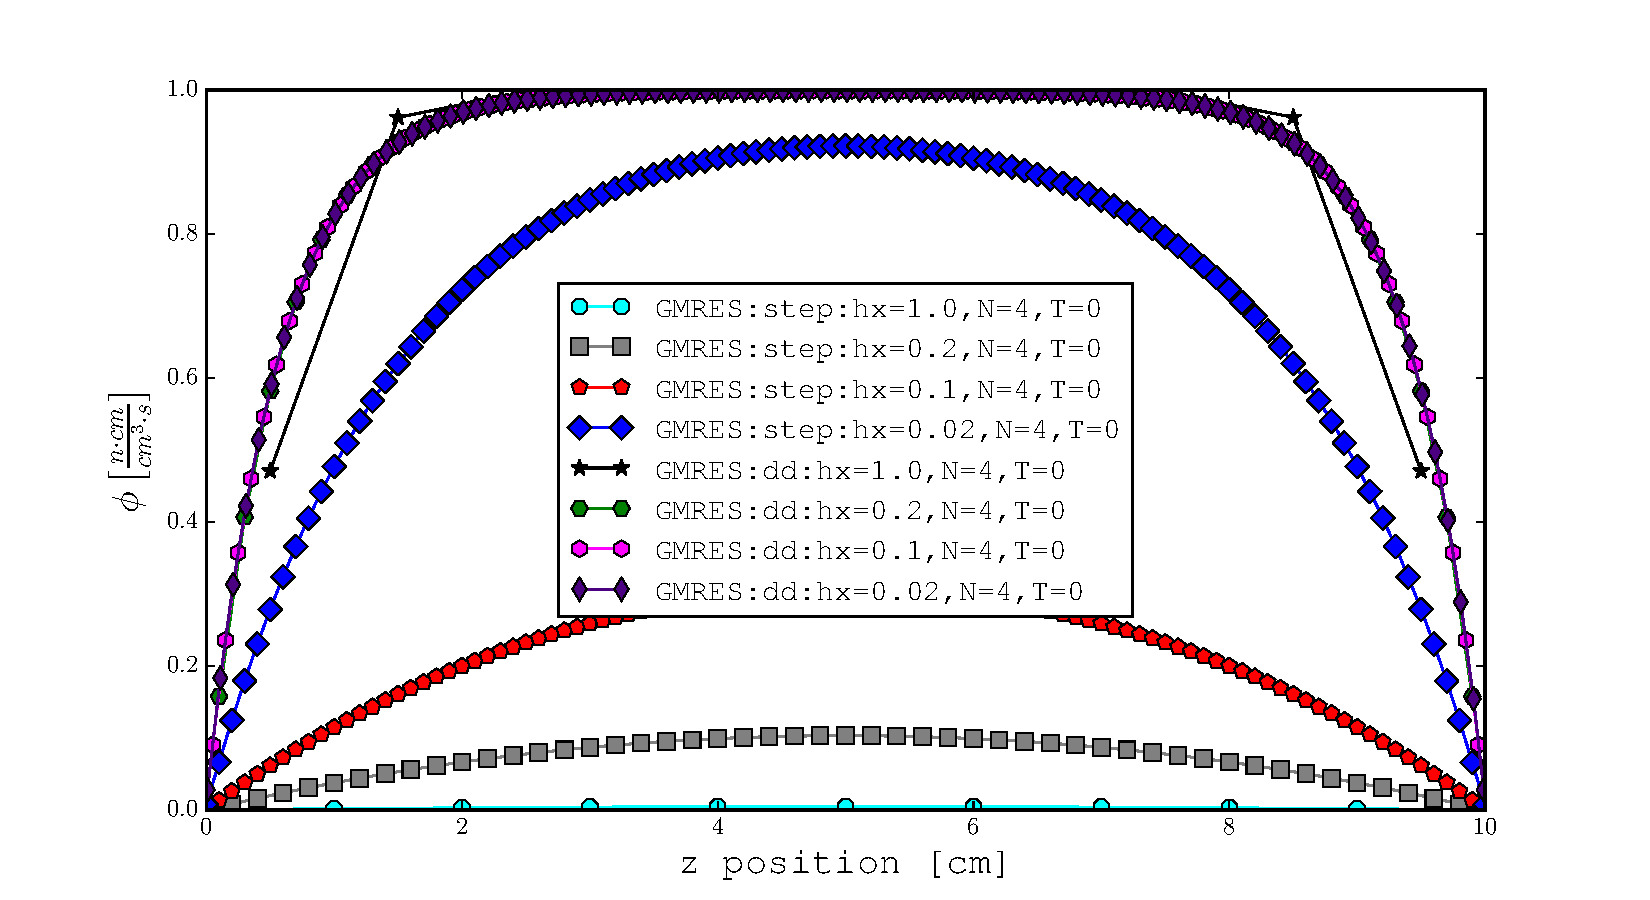
\includegraphics[width=1\columnwidth]
                      {Homework4/Plots/FluxPlot.pdf}
    \end{center}
  \end{figure}

  \textbf{Both of the iterative solutions converged with max iterations
  of 100,000 and a slight modification on cross section
  ($\bm{\Sigma_t=\Sigma_t\cdot1.0001}$) to help the system converge.
  As the number of zones increased
  for the step solution, the flux magnitude kept increasing to
  match with the diamond difference and maintained a cosine(ish)
  shape. As the number of zones increased with the diamond difference,
  the shape started to converge towards the cosine, but maintained
  the proper magnitude.}
  
  \textbf{Something else I would like to point out in the solution
    is that the step solution always had one more point plotted than the
    diamond difference. The reason for this is due to how each solution
    was solved. This is easier highlighted (for me) with an example,
    which is shown in the case
    where the number of zones is 10.}\\
  
  For the Diamond difference, the average locations (remember they were averaged),
  $\psi_{n,i}^{L,j+1}$, being solved for were,
  \begin{equation*}
    z=[0.5,1.5,2.5,3.5,4.5,5.5,6.5,7.5,8.5,9.5]
  \end{equation*}
  The points for $\psi_{n,i+1/2}^{L,j+1}$ and $\psi_{n,i-1/2}^{L,j+1}$ were at the points,
  \begin{equation*}
    z=[0,1,2,3,4,5,6,7,8,9,10]
  \end{equation*}
  When sweeping to the right, $\psi_{n}(z=0)$ was set to zero, because the incoming flux
  is zero, and all points were solved for up to where $z=10$, and $\psi_{n,i}$ values were
  determined with averaging. This same thing occured when sweeping to the left (except here $\psi_{n}(z=10)$ was set to zero). This would
  yield 10 values at the points $[0.5,1.5,...,9.5]$.\\

  For the step discretization scheme, the locations (non averaged), $\psi_{n,i}^{L,j+1}$, being solved for were,

  \begin{equation*}
    x=
    \begin{cases}
      [1,2,3,4,5,6,7,8,9,10] & \mu>0\\
      [0,1,2,3,4,5,6,7,8,9], & \mu<0
    \end{cases}
  \end{equation*}
  When combining these two lists for $\phi$, this was considered,
  and hence the step discretization scheme had one extra point (both
  lists have 10 points, but the location 10 is unqiue in the first list,
  and 0 in the second).
  
  \item{(10 points) Discuss why there is a different form of the
    discretization for the different signs of $\mu$.}

  \textbf{The different forms are needed in the step discretization because
  in both the diamond and step approaches to the solution a value is
  needed from a previous zone. Our vacuum boundary condition states
  that the incoming neutrons are zero, which at the left side of the
  boundary, determines the angular flux moving to the right, and at
  the right side of the boundary, the angular flux moving to the left
  (these values are 0).}

  \item{(40 points) Plot the error after each iteration using a 0
    initial guess for the step discretization with source iteration and
    GMRES.}

    \textbf{Error will be determined with the following:}
    \begin{equation*}
      \bm{\text{Error}=\frac{||\phi^{\ell+1}-
          \phi^\ell||}{||\phi^{\ell+1}||}}
    \end{equation*}

  \begin{figure}[H]
    \begin{center}
      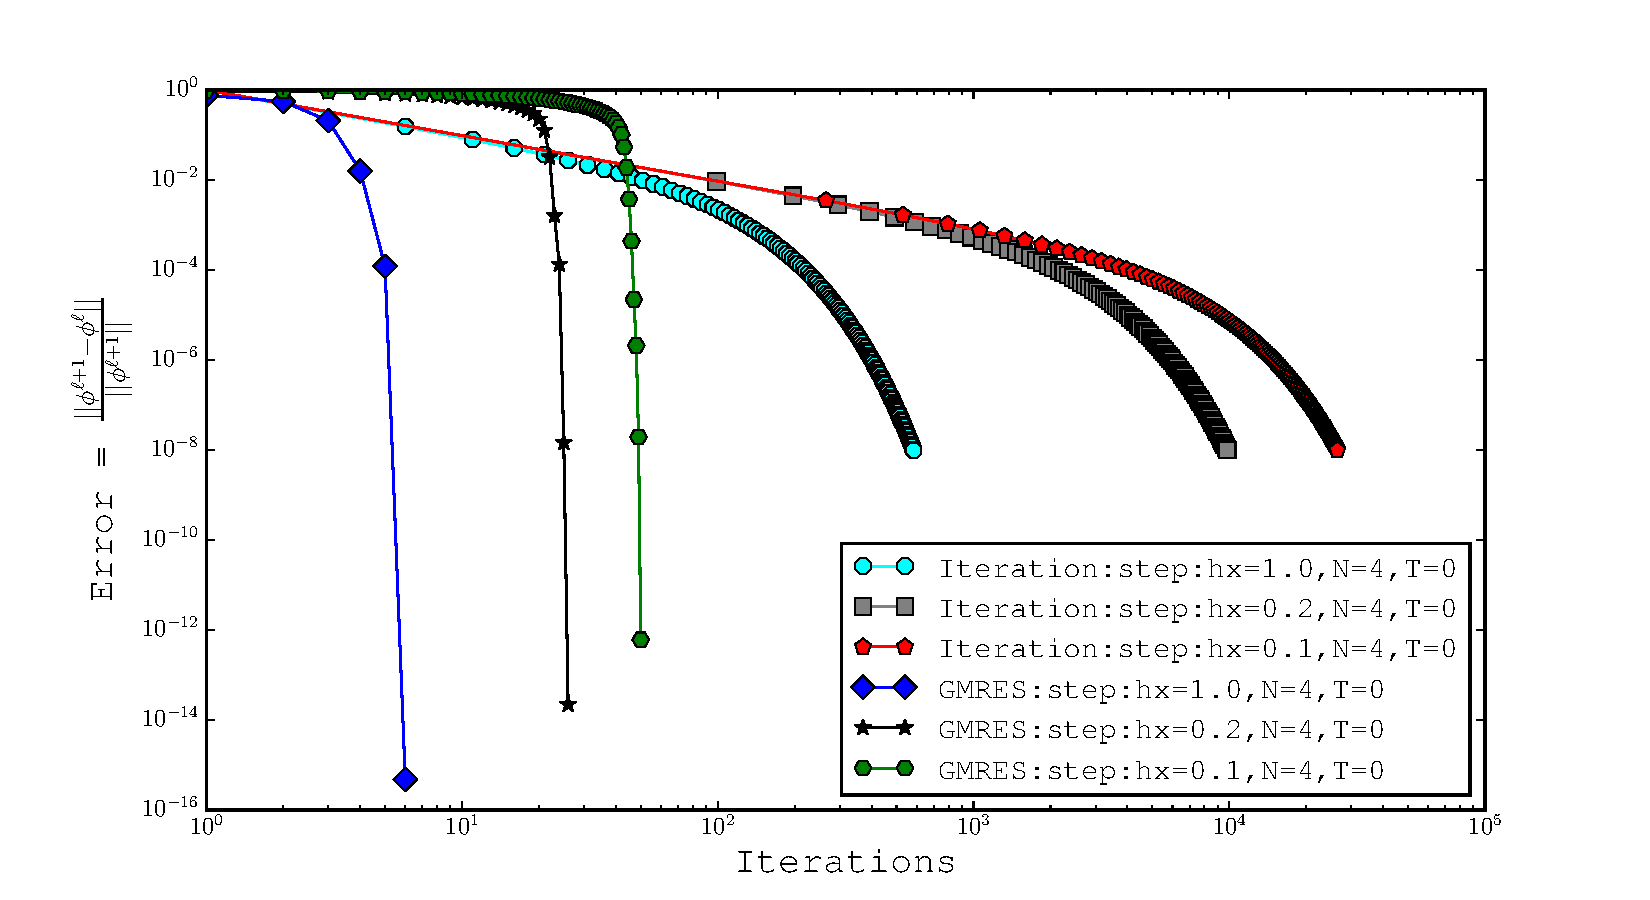
\includegraphics[width=1\columnwidth]
                      {Homework4/Plots/ErrorPlot.pdf}
    \end{center}
  \end{figure}
    
  \item{(50 points) Solve Reed's problem (see finite difference diffusion
    codes). Present convergence plots for the solution in space and angle
    to a ``refined'' solution in space and angle.}

    Plots are below, reduced the number of points so that figures
    wouldn't take so long to load.
  \begin{figure}[H]
    \begin{center}
      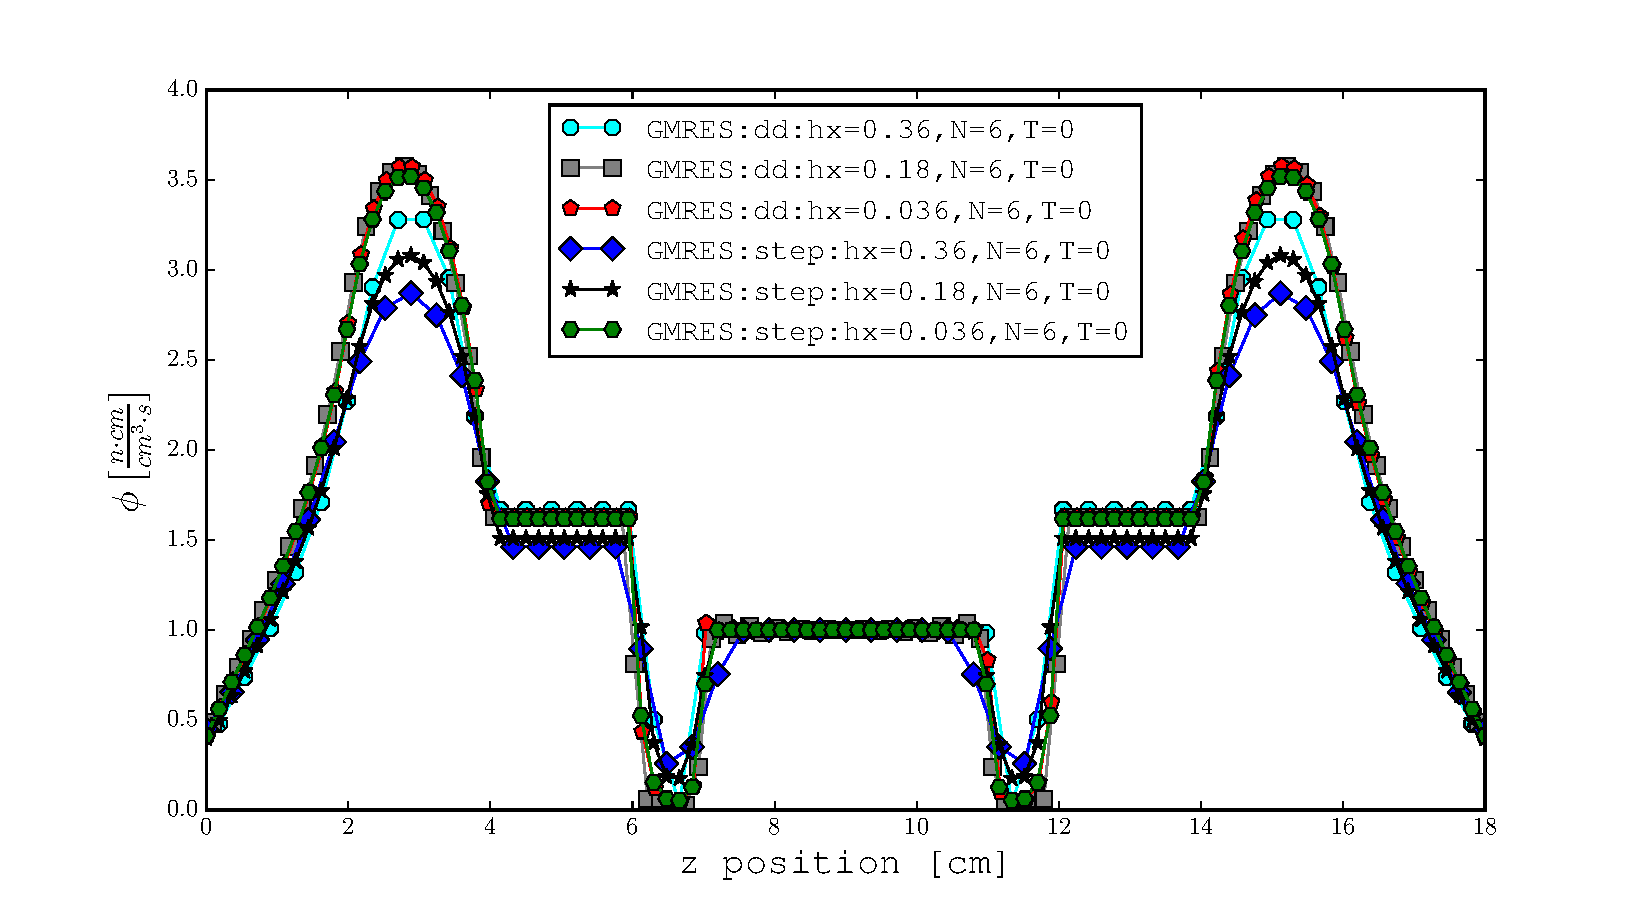
\includegraphics[width=1\columnwidth]
                      {Homework4/Plots/FluxPlotReed.pdf}
    \end{center}
  \end{figure}
  \begin{figure}[H]
    \begin{center}
      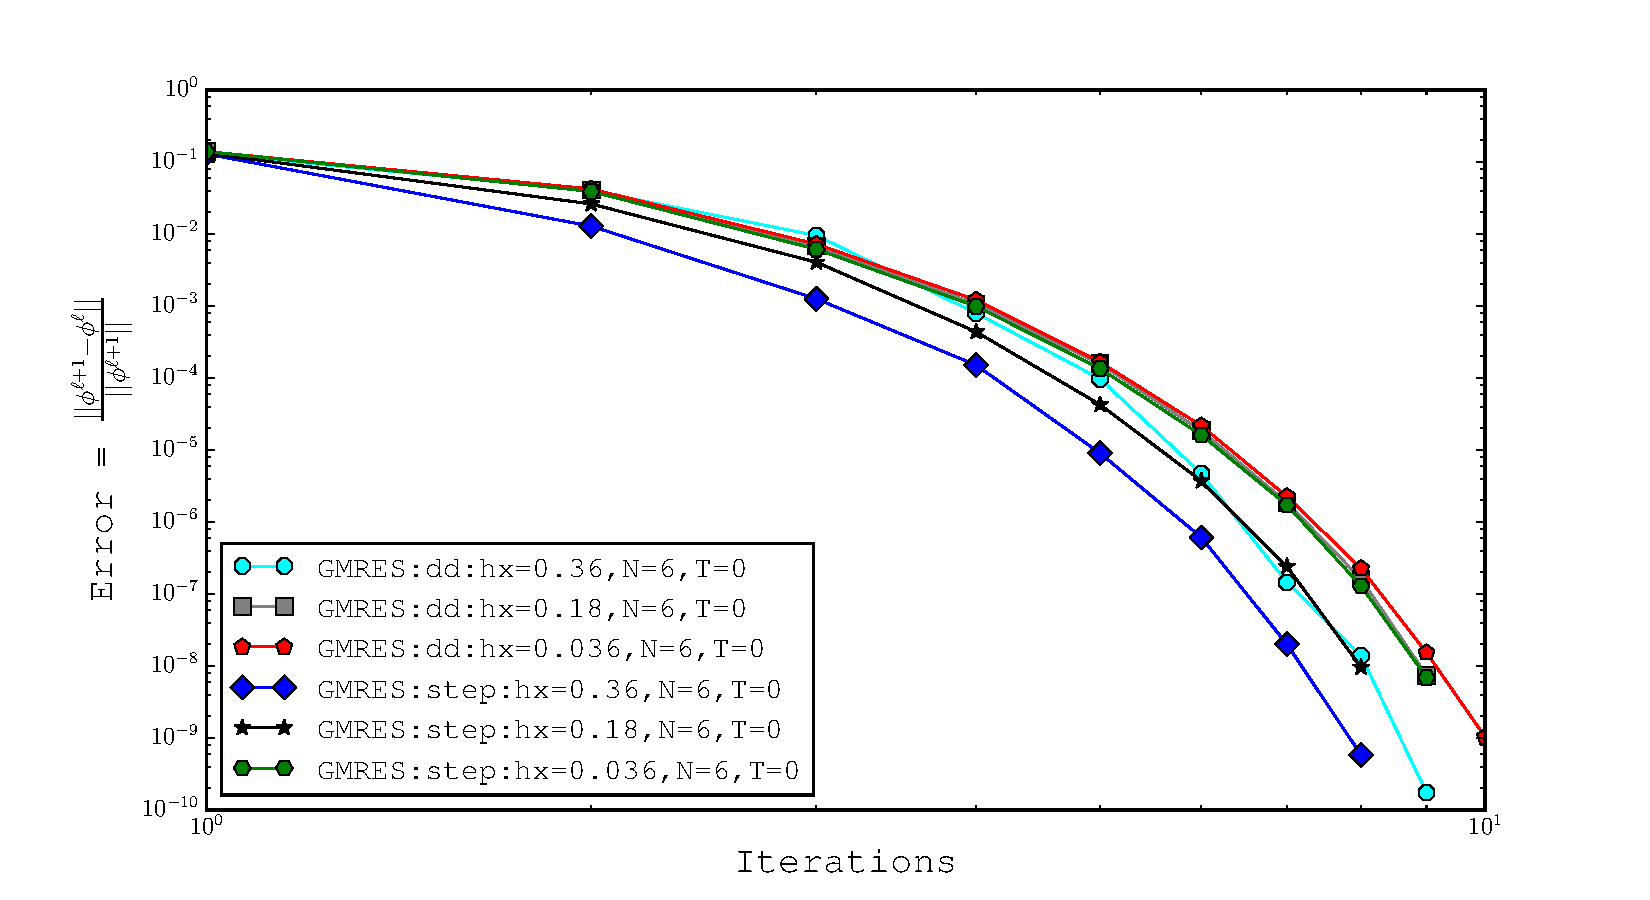
\includegraphics[width=1\columnwidth]
                      {Homework4/Plots/ErrorPlotReed.pdf}
    \end{center}
  \end{figure}
  \begin{figure}[H]
    \begin{center}
      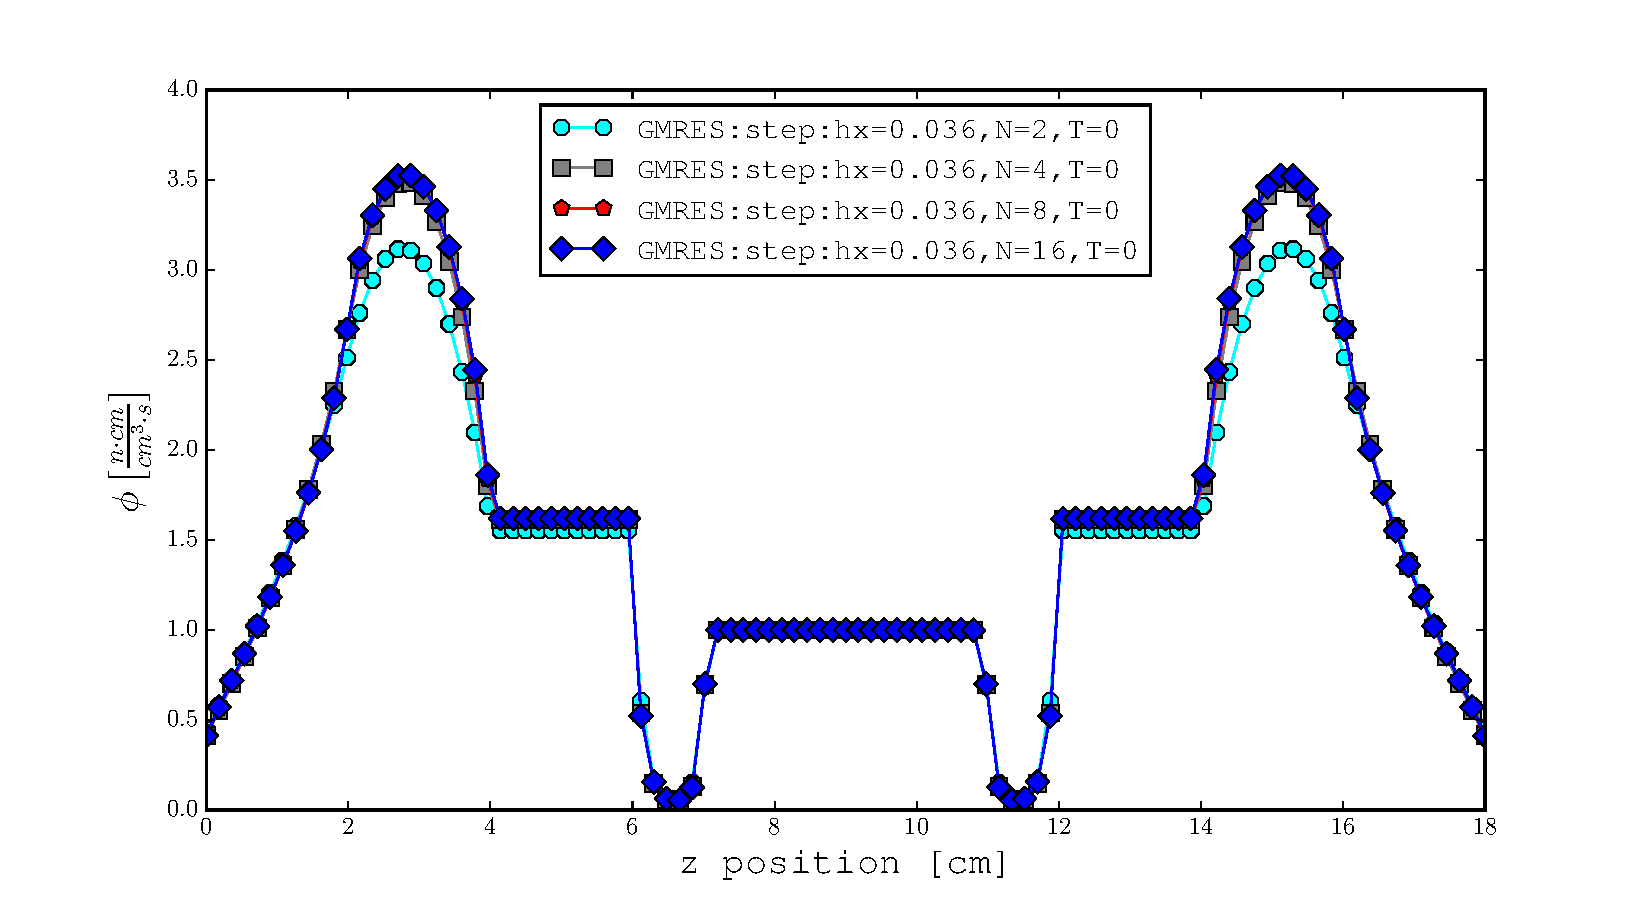
\includegraphics[width=1\columnwidth]
                      {Homework4/Plots/FluxPlotReedVaryN.pdf}
    \end{center}
  \end{figure}
  \begin{figure}[H]
    \begin{center}
      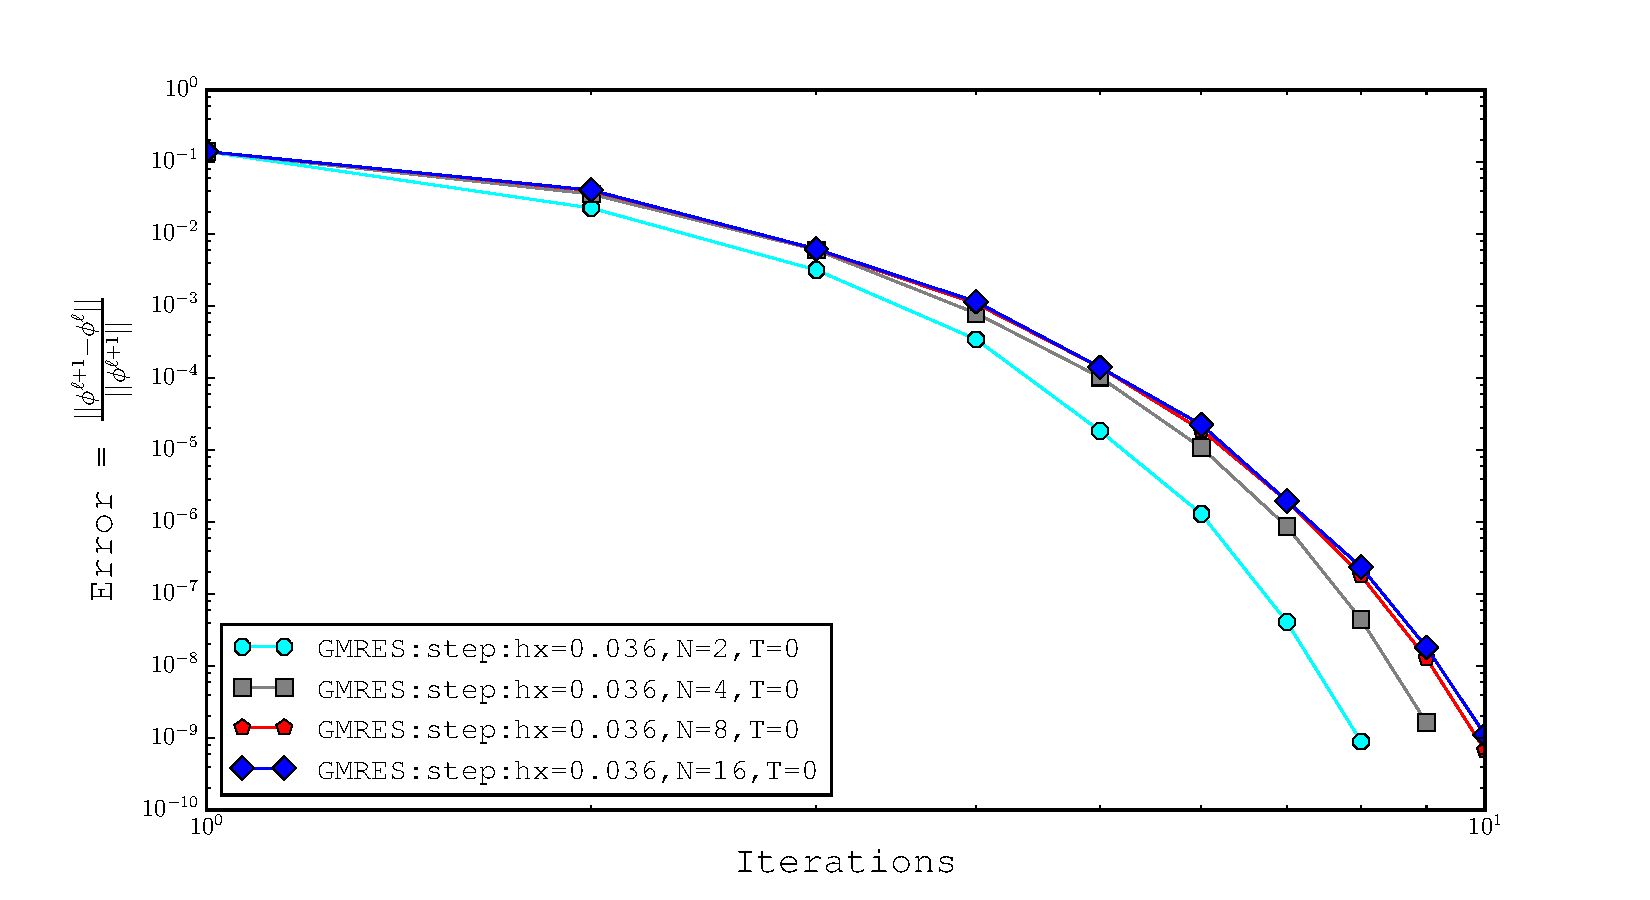
\includegraphics[width=1\columnwidth]
                      {Homework4/Plots/ErrorPlotReedVaryN.pdf}
    \end{center}
  \end{figure}

  The solution converges with more spatial slices. Increasing the
  number of angular slices helps upto when N=4, but beyond that
  it doesn't do much.
  
  \item{(50 points extra credit) Solve a time dependant problem for
    a slab surrounded by vacuum with $\Sigma_t=\Sigma_s=1$ and initial
    condition given by $\bm{\psi(0)=1/h_x}$ (original problem statement
    said $\phi(0)=1/h_x$ and I'm not sure how to solve that).
    Plot the solution at $t=1\ s$,
    using step and diamond difference. The particles have a speed of
    1 cm/s. Which discretization is better with a small time step?
    What do you see with a small number of ordinates compared to
    a really large number (100s)?}

  \begin{figure}[H]
    \begin{center}
      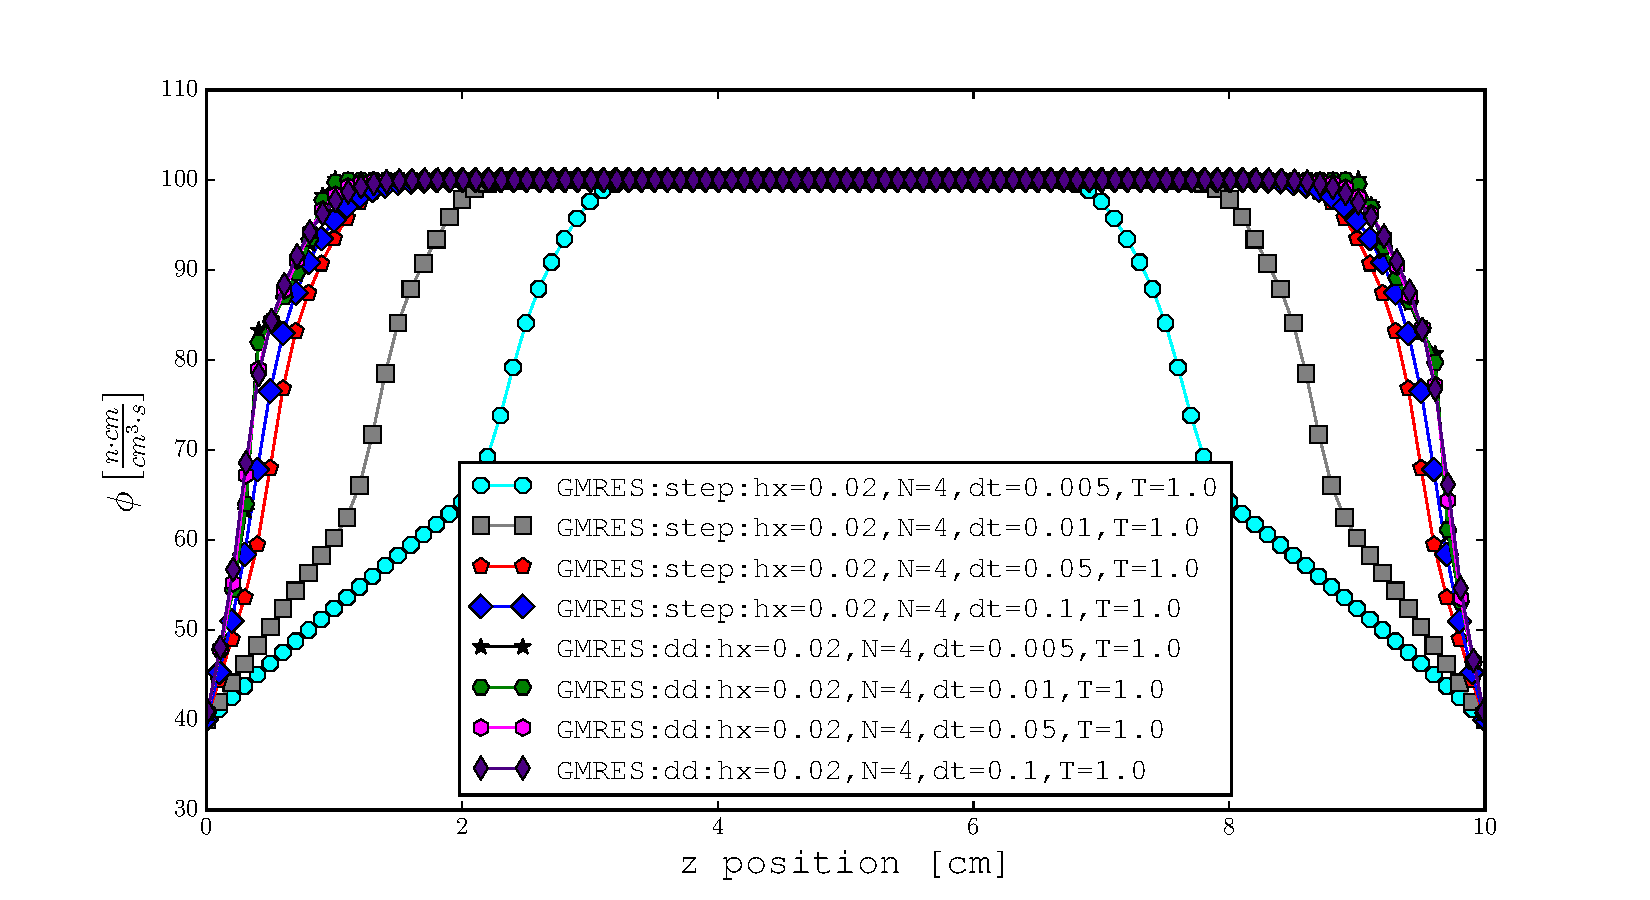
\includegraphics[width=1\columnwidth]
                      {Homework4/Plots/FluxPlotTime.pdf}
    \end{center}
    \caption{Q=0.01}
  \end{figure}
  \begin{figure}[H]
    \begin{center}
      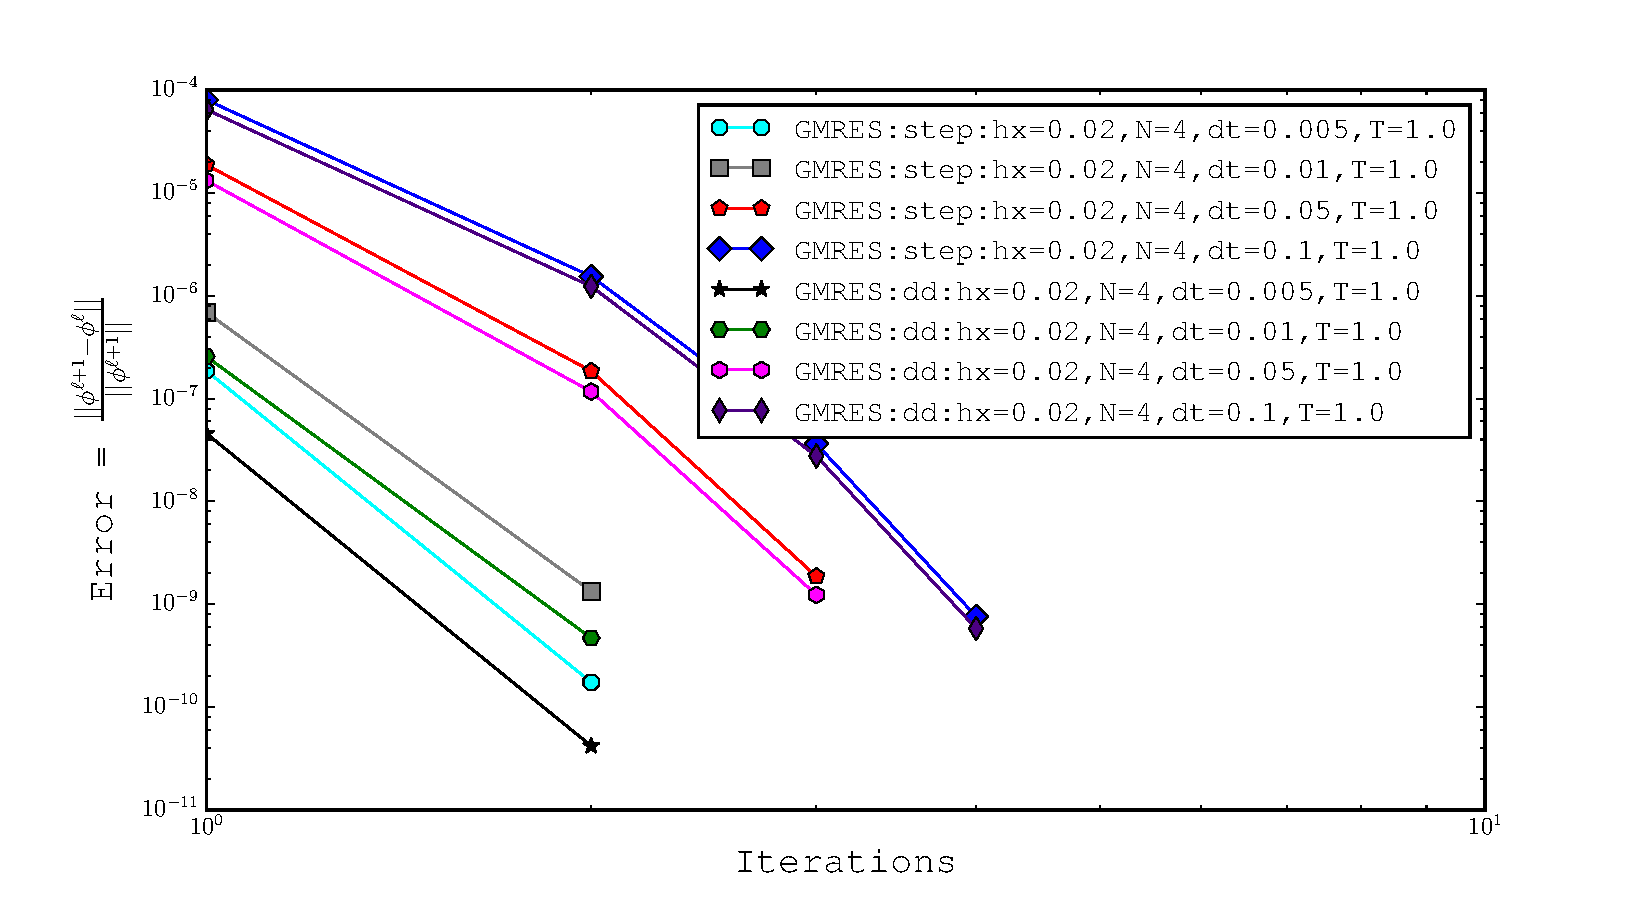
\includegraphics[width=1\columnwidth]
                      {Homework4/Plots/ErrorPlotTime.pdf}
    \end{center}
    \caption{Q=0.01}
  \end{figure}

  Based on the above graphs, I am not sure which solution does
  better with a smaller step size. It depends on what the answer
  should be. I think the step solution, as the step size increases,
  look like they have some nonphysical bends in the solution. This
  could be due to lots of things, but maybe its because of the smaller
  step size, which makes me think the diamond difference method is
  better with smaller step sizes.

  %% \begin{figure}[H]
  %%   \begin{center}
  %%     \includegraphics[width=1\columnwidth]
  %%                     {Homework4/Plots/FluxPlotTimeQ.pdf}
  %%   \end{center}
  %%   \caption{Q=0}
  %% \end{figure}
  %% \begin{figure}[H]
  %%   \begin{center}
  %%     \includegraphics[width=1\columnwidth]
  %%                     {Homework4/Plots/ErrorPlotTimeQ.pdf}
  %%   \end{center}
  %%   \caption{Q=0}
  %% \end{figure}

  
  \begin{figure}[H]
    \begin{center}
      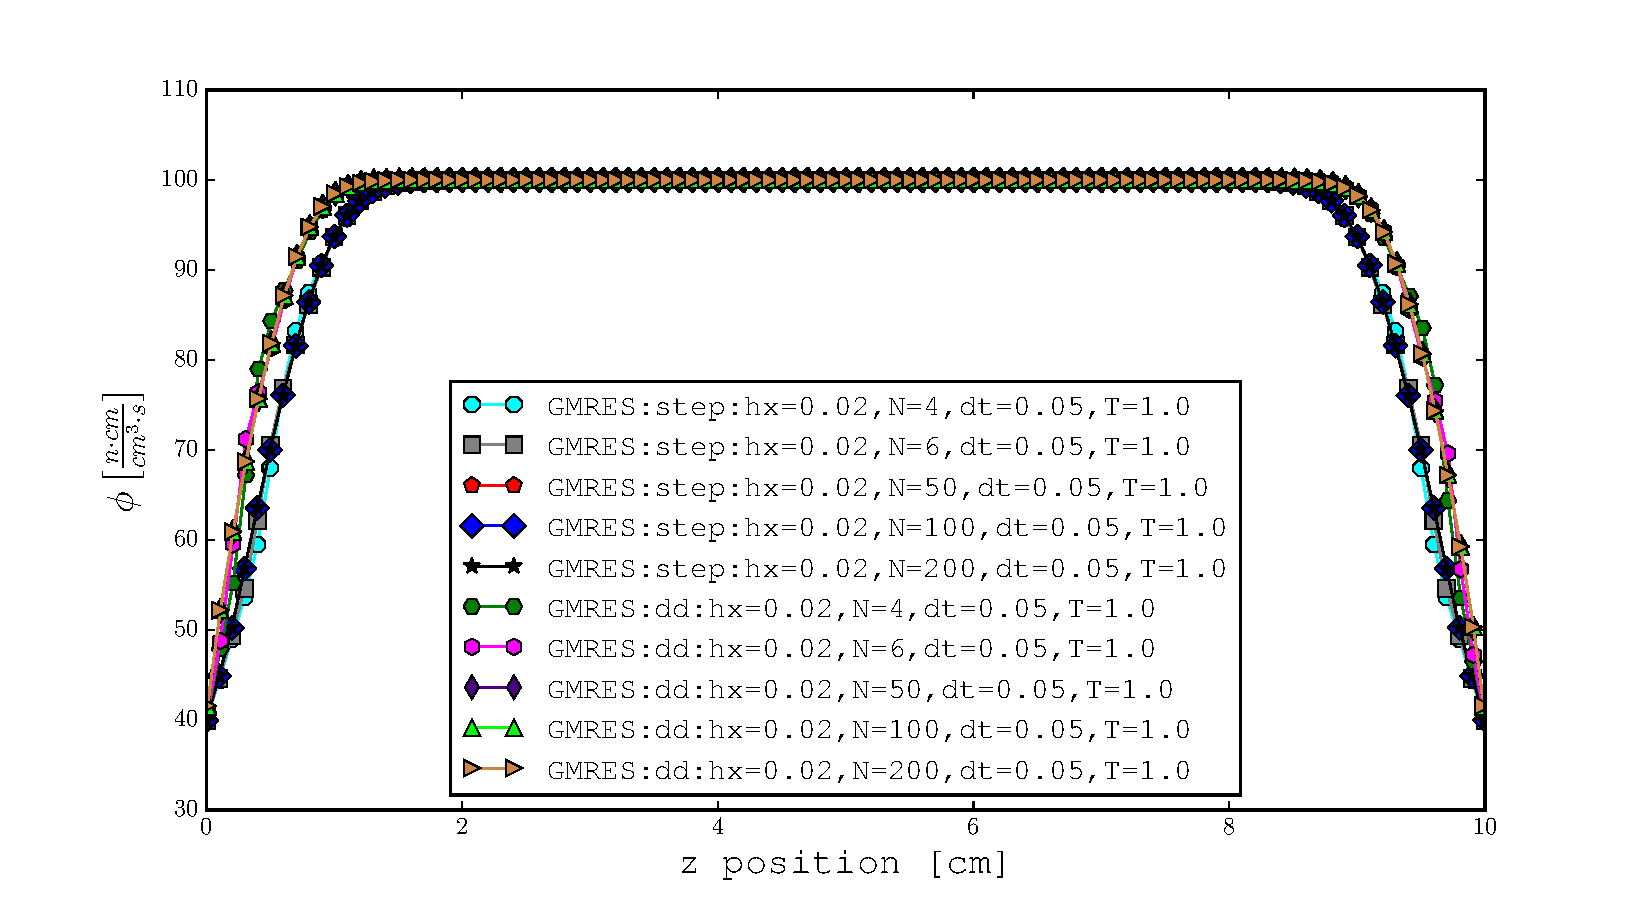
\includegraphics[width=1\columnwidth]
                      {Homework4/Plots/FluxPlotTimeVaryN.pdf}
    \end{center}
  \end{figure}
  \begin{figure}[H]
    \begin{center}
      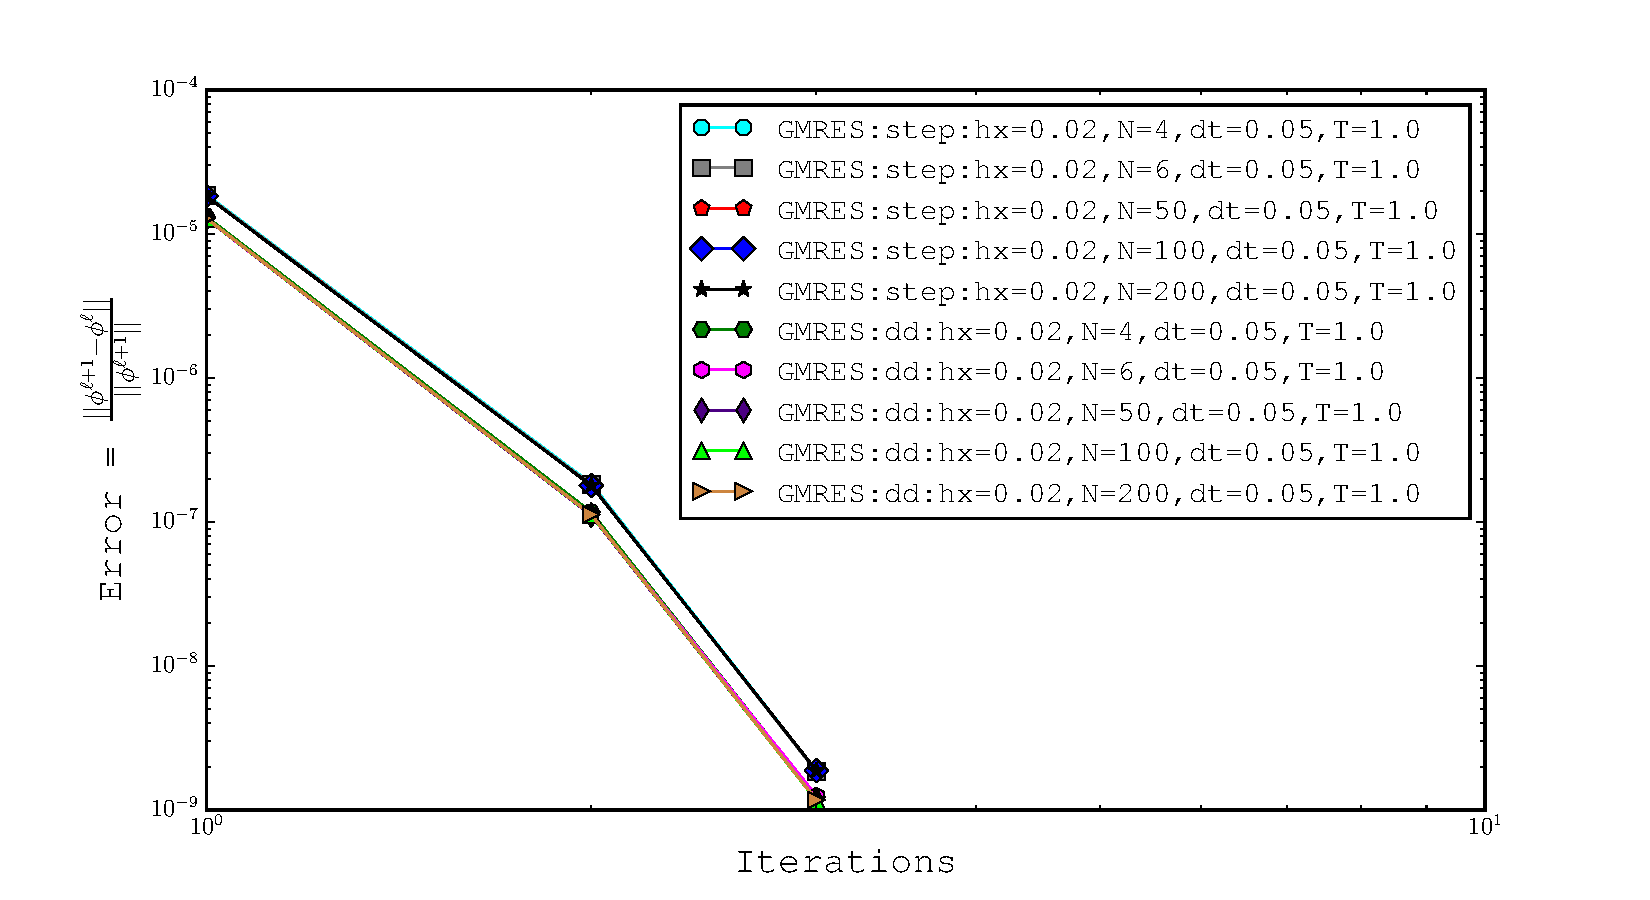
\includegraphics[width=1\columnwidth]
                      {Homework4/Plots/ErrorPlotTimeVaryN.pdf}
    \end{center}
  \end{figure}

  As the number of ordinances increase in the problem there
  isn't much change in the solution, which is expected because
  with the Quadrature rule we used, the integral can usually
  be expressed within around 6 terms. There was an increase
  in computational time though.
  
  \end{enumerate}
           
\end{homeworkProblem}
\clearpage

%--------------------------------------------------------------------------
%	Homework 4 Code
%--------------------------------------------------------------------------

\begin{homeworkProblem}[Homework 4 Code]
    
  \pythonscript{Homework4/Calculations}
               {\textbf{Main Code For Parts a,b and c}}
  \pythonscript{Homework4/CalculationsP4}
               {\textbf{Main Code For Part d}}
  \pythonscript{Homework4/CalculationsP5}
               {\textbf{Main Code For Part e}}
  \pythonscript{Homework4/Functions.py}
               {\textbf{Functions holder}}
  
\end{homeworkProblem}

\clearpage

%--------------------------------------------------------------------------
%	Homework 5 Problem Statement
%--------------------------------------------------------------------------

\begin{homeworkProblem}[Homework 5 Problem Statement]
  Solve the following problem and submit a detailed report,
  including a justification of why a reader should believe your
  results.\\

  \textbf{Clean Fusion Energy}\\

  (100 points) Consider a thermonuclear fusion reactor producing
  neutrons of energy 14.1 and 2.45 MeV. The reactor is surrounded
  by
  \href{https://en.wikipedia.org/wiki/FLiBe}{FLiBe}
  (a 2:1 mixture of LiF and BeF\tsbs{2}) to convert
  the neutron energy into heat. All the constituents in the
  FLiBe have their natural abundances. Using data from
  \href{https://www.oecd-nea.org/janis/}{JANIS}, and assuming
  the total neutron flux is 10\tss{14} n/cm\tss{2}$\cdot$s.
  Perform the following analyses.
  \begin{enumerate}[label=(\alph*)]
  \item{(25 points) Write out the depletion (or in thise case
    activation) chains that will occur in the system.}
  \item{(50 points) Over a two-year cycle compute the inventory
    of nuclides in the system using two methods discussed in class.
    What is the maximum concentration of tritium?}
  \item{(25 points) After discharging the FLiBe blanket, how long
    will it take until the material is less radioactive than
\href{http://www.orau.org/PTP/collection/consumer%20products/brazilnuts.htm}{Brazil Nuts}
    ? (444 Bq/kg)
    }
  \end{enumerate}
\end{homeworkProblem}

\clearpage

%--------------------------------------------------------------------------
%	Homework 5 Background
%--------------------------------------------------------------------------

\begin{homeworkProblem}[Homework 5 Background]
  Please note, that most of this background is copied directly from
  Dr. McClarren's notes, but are reproduced here.\\~\\

  The production of an isotope is dictated by production and loss
  \begin{equation*}
    \frac{dn_i}{dt}=-\lambda_i^{eff}n_i+
    \sum_{j=1}^{N}b_{j\rightarrow i}^{eff}\lambda_j^{eff}n_j
  \end{equation*}
  Where,
  \begin{equation*}
    \lambda_i^{eff}=\lambda_i+\phi\sum_{j=1}^N\sigma_{i\rightarrow j}
  \end{equation*}
  and
  \begin{equation*}
    b_{j\rightarrow i}^{eff}=\frac{b_{j\rightarrow i}\lambda_j+
      \sigma_{j\rightarrow i}\phi}{\lambda_{j}^{eff}}
  \end{equation*}
  For a system of isotopes, this can be reduced to:
  \begin{equation*}
    \frac{d\vec{n}}{dt}=\bm{A}\vec{n}(t)
  \end{equation*}
  Where $\bm{A}$ is a matrix whose diagonal elements are
  $[-\lambda_1^{eff},-\lambda_2^{eff},...,-\lambda_N^{eff}]$,
  all off diagonal elements are
  $b_{j\rightarrow i}^{eff}\lambda_j^{eff}$ (i for the diagonal, and j is
  for the off diagonal position) and $\vec{n}(t)=[n_1,n_2,...,n_N]$.\\

  The solution to this system is obvious (it wasn't to me at first - but
  that's because I'm a newb)
  
  \begin{equation*}
    \vec{n}=e^{\bm{A}t}\vec{n}_0
  \end{equation*}

  Determing $e^{\bm{A}t}\vec{n}_0$ will be done 3 different ways,\\

  \textbf{Matrix Exponential}\\
  
  Analytic Solution, unstable with large N.
  \begin{equation*}
    \vec{n}(t)=e^{\bm{A}t}\vec{n}_0\approx\left[
    \sum_{m=0}^\infty\frac{1}{m!}\bm{A}^mt^m\right]\vec{n}_0
  \end{equation*}
  \\
  \textbf{Backward Euler}\\
  
  Unstable for large $\Delta t$, but can take time steps.
  \begin{align*}
    \frac{d\vec{n}}{dt}\approx
    \frac{\vec{n}(\Delta t)-\vec{n}_0}{\Delta t}\approx
    &\bm{A}\vec{n}(\Delta t)\\
    \vec{n}(\Delta t)\approx&(\bm{I}-\bm{A}\Delta t)^{-1}\vec{n}_0
  \end{align*}
  \textbf{Rational Approximation}
  \begin{align*}
    \vec{n}(t)=e^{\bm{A}t}\vec{n}_0\approx-2\Re\sum_{k=1}^{N/2}c_k
    (z_k\bm{I}-\bm{A}t)^{-1}\vec{n}_0
  \end{align*}
  with
  \begin{equation*}
    c_k=\frac{i}{N}e^{z_k}w_k
  \end{equation*}
  where $z_k$ and $w_k$ are both scalers defined as
  \begin{align*}
    z_k=&\phi(\theta_k)\\
    w_k=&\phi'(\theta_k)
  \end{align*}
  with
  \begin{align*}
    \phi(\theta)=&N[0.1309-0.1194\theta^2+0.2500i\theta]\\
    &\text{or}\\
    \phi(\theta)=&N[0.5071\theta cot(0.6407\theta)-0.6122+0.2645i\theta]
  \end{align*}
  and
  \begin{equation*}
    \theta_k=\pm\frac{\pi}{N}\left(1+2k\right)\ \ \text{k from 0 to N-1}
  \end{equation*}
  Where $N$ doesn't have to go much higher than 10 to have low errors.
\end{homeworkProblem}

\clearpage



%--------------------------------------------------------------------------
%	Homework 5 Solution
%--------------------------------------------------------------------------

\begin{homeworkProblem}[Homework 5 Solution]
  \begin{enumerate}[label=(\alph*)]
  \item{(25 points) Write out the depletion (or in thise case
    activation) chains that will occur in the system.}\\~\\
    
    The chains were written out in a form so that the diagram would
    be uncluttered, and not all possible reactions are displayed.
    
    \begin{figure}[H]
      \begin{center}
        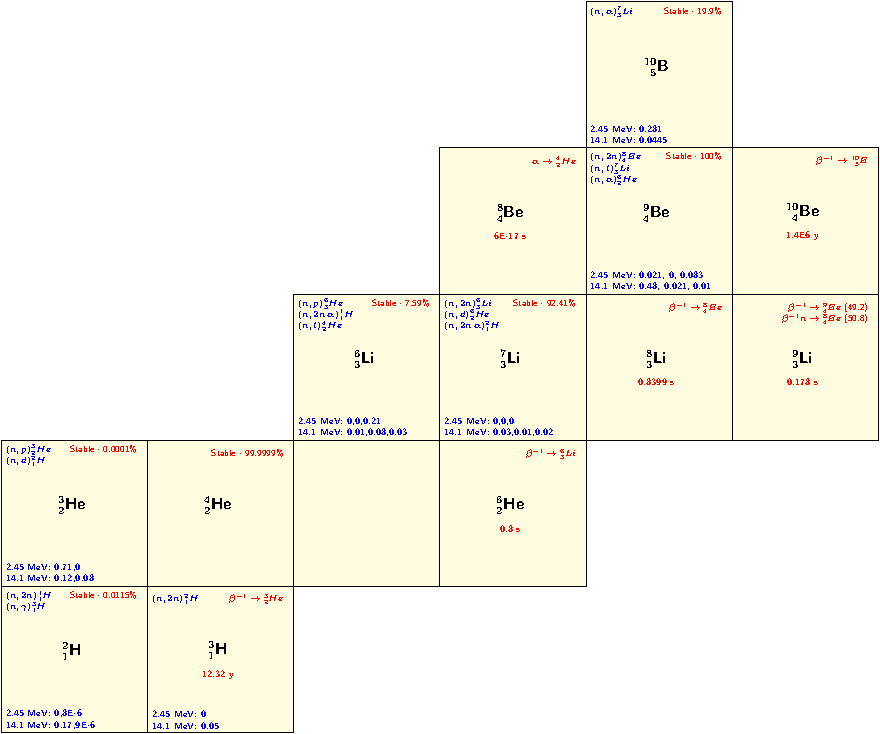
\includegraphics[width=1\columnwidth]{BeLi.pdf}
      \end{center}
    \end{figure}
    
    \begin{figure}[H]
      \begin{center}
        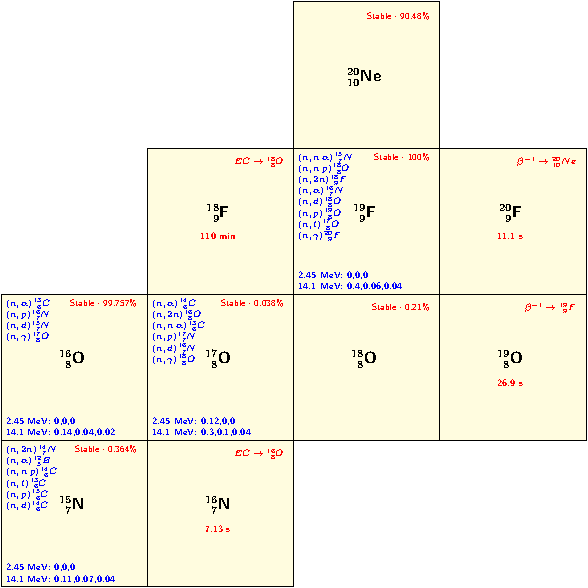
\includegraphics[width=1\columnwidth]{FO.pdf}
      \end{center}
    \end{figure}


    
  \item{(50 points) Over a two-year cycle compute the inventory
    of nuclides in the system using two methods discussed in class.
    What is the maximum concentration of tritium?}
  \item{(25 points) After discharging the FLiBe blanket, how long
    will it take until the material is less radioactive than
\href{http://www.orau.org/PTP/collection/consumer%20products/brazilnuts.htm}{Brazil Nuts}
    ? (444 Bq/kg)
    }
  \end{enumerate}
\end{homeworkProblem}

\clearpage


%--------------------------------------------------------------------------
%	Project
%--------------------------------------------------------------------------

\begin{homeworkProblem}[Project]

  \problemAnswer{
    
  }
  
\end{homeworkProblem}

\clearpage



  %% \begin{equation*}
  %%   u(x,0)=
  %%   \begin{cases}
  %%     1, & x\in[0,2.5]\\
  %%     0, & \text{otherwise}
  %%   \end{cases}
  %% \end{equation*}


  
  %% \begin{enumerate}[label=(\alph*)]
  %% \item{$\mu_v=0.5,\ \sigma_c=0.1$}
  %% \item{$\mu_D=0.125,\ \sigma_D=0.03$}
  %% \item{$\mu_\omega=0.1,\ \sigma_\omega=0.05$}
  %% \end{enumerate}
  %% How do these results change with changes in $\Delta x$ and $\Delta t$?\\~\\

  
  %% \pythonscript{Problem4_long/Calc2}{Code for Problem - run many times}
  
  %% \begin{figure}[H]
  %%   \begin{center}
  %%     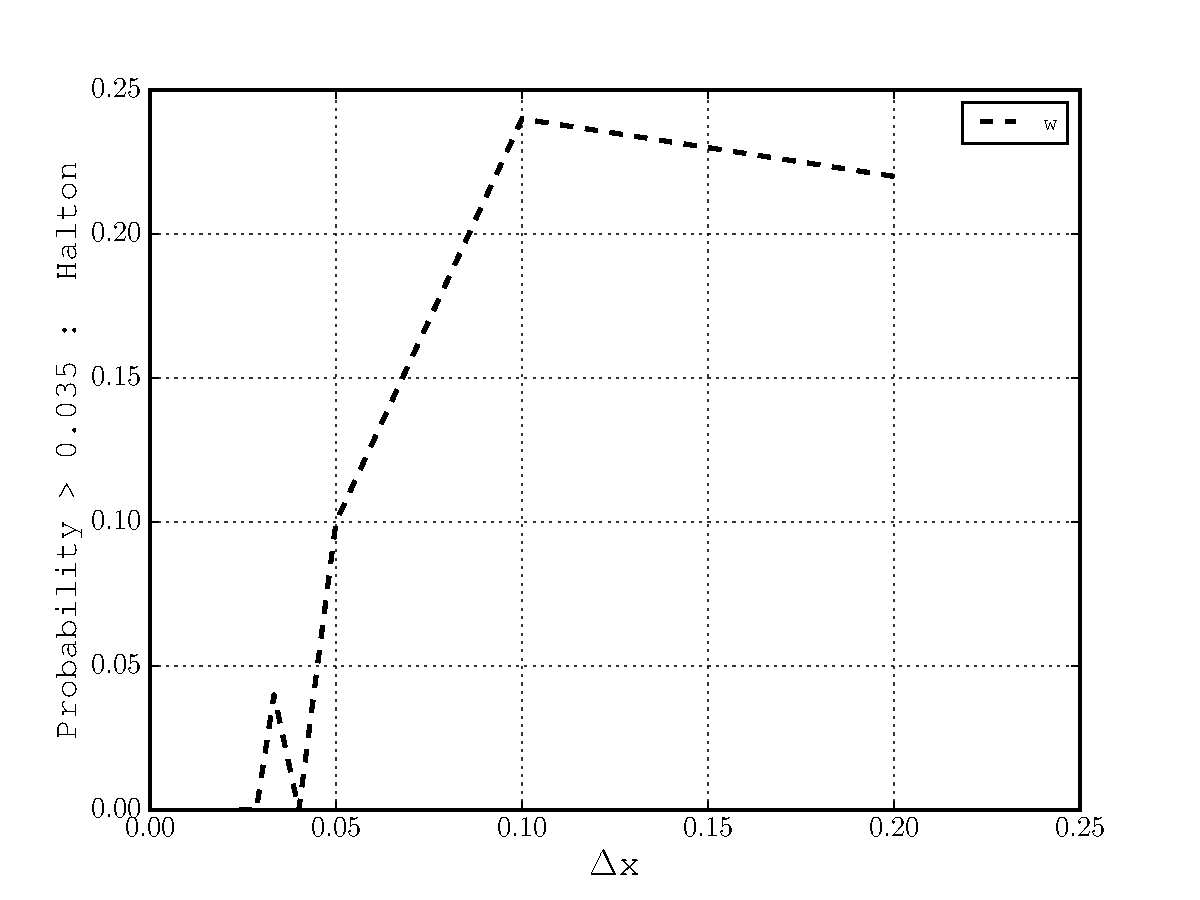
\includegraphics[width=0.77\columnwidth]{Problem4_long/Halton_wx.pdf}
  %%   \end{center}
  %% \end{figure}


  %% \begin{table}[H]
  %%   \begin{center}
  %%     \caption{Sensitivity Parameters dx = 0.1 dt = 0.5}
  %%     \begin{tabular}{l l l l l}
  %%       \toprule
  %%       Variable & Coef & Std Err & t-stat & p-value\\
  %%       \hline
  %%       $v$        &  0.1945  & 8.5335  &  0.02 & 0.9818\\
  %%       $D$        & -25.2844 & 33.3347 & -0.76 & 0.4483\\
  %%       $w$        &  76.5716 & 42.3267 & 1.81  & 0.0707\\
  %%       $\Delta t$ & -7.2201  & 1.8227  & -3.96 & 0.0001\\
  %%       $\Delta x$ &  30.8771 & 2.6986  & 11.44 & 0.0000\\
  %%       \hline
  %%       intercept & -5.1421 & 7.2558 & -0.71 & 0.4787\\
  %%       \bottomrule
  %%     \end{tabular}
  %%   \end{center}
  %% \end{table}

%\pythonscript{Problem1/Calculations}{Script for Problem}
%% \begin{figure}[H]
%%   \begin{center}
%%     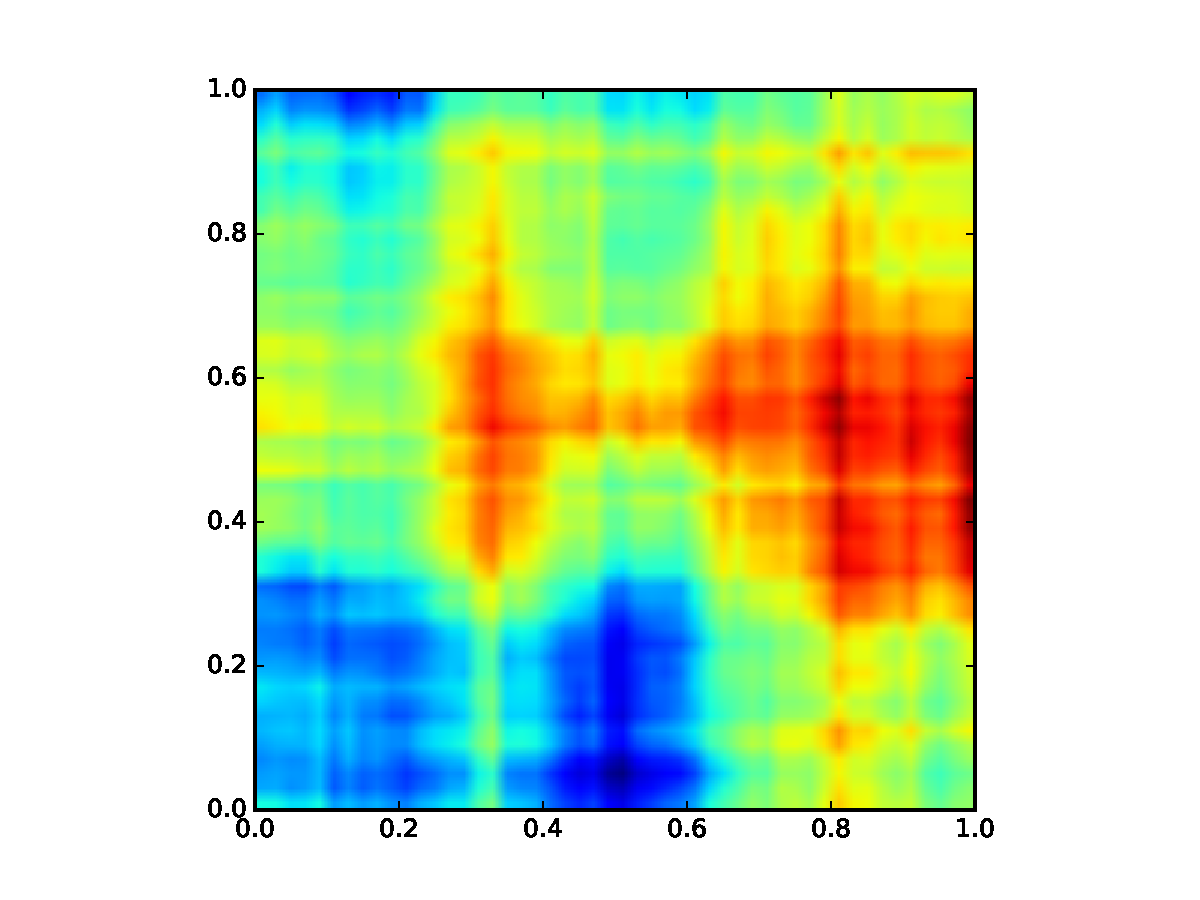
\includegraphics[width=0.77\columnwidth]{Problem1/P1realization1.pdf}
%%   \end{center}
%% \end{figure}
%\problemAnswer{TADA}

%--------------------------------------------------------------------------
%% This is an example citation \cite{Tatro2013}.
%% \bibliography{references} 
%% \bibliographystyle{plain} 

\end{document}
